\documentclass{article}
\usepackage[polish]{babel}
\usepackage[T1]{fontenc}
\usepackage[utf8]{inputenc}
\usepackage{graphicx}
\usepackage{float}
\usepackage[bottom=0.5cm, right=1.5cm, left=1.5cm, top=1.5cm]{geometry}
\graphicspath{{../pliki}}



\title{%
  Cyberbezpieczeństwo - laboratoria 3 \\
  \large Blokowe algorytmy szyfrujące}
\author{Patryk Łuszczek 272707}
\date{\today}
\begin{document}
\maketitle
\newpage
\tableofcontents
\newpage

\section{Przykładowe algorytmy blokowe}
Do analizy własności algorytmów zostały wykorzystane trzy teksty o różnym stopniu zróżnicowania:
\begin{itemize}
    \item \textbf{Jednolity:} znak "G" powtórzony 1000 razy
    \item \textbf{Średnio zróżnicowany:} zdanie "Norse Nordic or Scandinavian mythology is the body of myths belonging to the North Germanic peoples" powtórzone 10 razy
    \item \textbf{Zróżnicowany:} 
    Descriptions of Cerberus vary including the number of his heads Cerberus was usually threeheaded though not always Cerberus had several multiheaded relatives His father was the multi snakefooted Typhon and Cerberus was the brother of three other multiheaded monsters the multisnakeheaded Lernaean Hydra Orthrus the twoheaded dog that guarded the Cattle of Geryon and the Chimera who had three heads that of a lion a goat and a snake And like these close relatives Cerberus was with only the rare iconographic exception multiheaded In the earliest description of Cerberus Hesiods Theogony c 8th  7th century BC Cerberus has fifty heads while Pindar c 522  c 443 BC gave him one hundred heads However later writers almost universally give Cerberus three heads An exception is the Latin poet Horaces Cerberus which has a single dog head and one hundred snake heads Perhaps trying to reconcile these competing traditions Apollodoruss Cerberus has three dog heads and the heads of all sorts of snakes along his back while the Byzantine poet John Tzetzes who probably based his account on Apollodorus gives Cerberus fifty heads three of which were dog heads the rest being the heads of other beasts of all sorts
\end{itemize}
Użycie tekstów o różynch stopniach zróżnicowania umożliwy dokładniejszą analizę algorytmów.

Badaniu zostały poddane trzy algorytmy blokowe:
\begin{itemize}
    \item \textbf{IDEA} - algorytm operujący na 64-bitowych blokach tekstu, wykorzystuje 128-bitowy klucz
    \item \textbf{Triple DES} - algorytm operujący na 64-bitowych blokach, wykonuje szyfrowanie DES trzykrotnie, wykorzystuje 128-bitowy klucz
    \item \textbf{AES} - algorytm operujący na 128-bitowych blokach, oferuje różne możliwości długości klucza (128, 192 lub 256 bitowy)
\end{itemize}
Ponadto w przypadku algorytmu 3DES w oprogramowaniu CrypTool istnieje możliwość szyfrowania w dwóch trybach:
\begin{itemize}
    \item \textbf{ECB (Electronic Codebook):} - szyfrowanie i deszyfrowanie każdego bloku tekstu oddzielnie, umożliwia to wykorzystanie wielu wątków równocześnie 
    \item \textbf{CBC (Cipher-Block Chaining):} - dodaje dodatkową "warstwę" bezpieczeństwa, poprzez wykonywanie operacji XOR na kolejnych blokach tekstu względem poprzednio zaszyfrowanego bloku. W wyniku tej zależności między blokami szyfru nie jest możliwe wykorzystanie wielu wątków jednocześnie - cały tekst musi zostać poddany procesie szyfrowania
\end{itemize}
\subsection{Zadanie 1.1}
    Klucz użyty do szyfrowania: \textbf{1A 3E BF 95 0A 5B 12 EF 78 CC B6 8B 66 31 6B FA}
    \begin{table}[H]
        \centering
        \caption{Porównanie entropii dla różnych algorytmów}
        \begin{tabular}{|c|c|c|c|}
        \hline
        Algorytm / Tekst & Jednolity & Średnio zróżnicowany & Wysoko zróżnicowany  \\ \hline
        Tekst jawny & 0.00 & 4.02 & 4.11 \\  \hline
        IDEA & 2.87 & 7.05 & 7.83  \\  \hline
        3DES (ECB) & 3.06  & 7.07 & 7.84 \\ \hline
        AES & 7.83 & 7.83 & 7.84 \\  \hline
        \end{tabular}
    \end{table}
    Jak można zauważyć algorytm AES cechuje się wprowadzeniem największej losowości znaków w szyfrogramie. Można to dostrzec
    przede wszystkim dla tekstu jednolitego i średnio zróżnicowanego. W przypadku tekstu wysocezróżnicowanego, wyszystkie testowane algorytmy
    cechują się entropią szyfrogramu na bardzo przybliżonym poziomie.
\subsection{Zadanie 1.2}
W celu przetestowania algorytmów w zależności od długości klucza, został wykorzystany klucz: \textbf{1A 3E BF 95 0A 5B 12 EF 78 CC B6 8B 66 31 6B FA AF B6 13 66 B8 6B CC 87 FE 21 B5 A0 95 FB E3 A1}, z którego był brane kolejne bajty w zależności od 
ustawienia algorytmu. Analizie został poddany tekst jednolity i średnio zróżnicowany.
    \begin{table}[H]
        \caption{Algorytm RC2}
        \centering
        \begin{tabular}{|c|c|c|}
            \hline
            Bity klucza & Jednolity & Średnio zróżnicowany \\ \hline
            8 & 7.78 & 7.80 \\ \hline
            16 & 7.78 & 7.79 \\ \hline
            32 & 7.79 & 7.81 \\ \hline
            64 & 7.78 & 7.79 \\ \hline
            128 & 7.79 & 7.80 \\ \hline
        \end{tabular}
    \end{table}

    \begin{table}[H]
        \caption{Algorytm RC4}
        \centering
        \begin{tabular}{|c|c|c|}
            \hline
            Bity klucza & Jednolity & Średnio zróżnicowany \\ \hline
            8 & 7.78 & 7.81 \\ \hline
            16 & 7.79 & 7.80 \\ \hline
            32 & 7.81 & 7.80 \\ \hline
            64 & 7.83 & 7.79 \\ \hline
            128 & 7.80 & 7.79 \\ \hline
        \end{tabular}
    \end{table}

    \begin{table}[H]
        \caption{Algorytm AES}
        \centering
        \begin{tabular}{|c|c|c|}
            \hline
            Bity klucza & Jednolity & Średnio zróżnicowany\\ \hline
            128 & 7.83 & 7.83 \\ \hline
            192 & 7.80 & 7.80 \\ \hline
            256 & 7.77 & 7.82 \\ \hline
        \end{tabular}
    \end{table}
    Jak można zauważyć, entropia szyfrogramów była bardzo wysoka dla każdej długości klucza.
\subsection{Pytanie 1.3}
    \textbf{Treść:} Gdzie obecnie są stosowane algorytmy blokowe? Które algorytmy \\\\
    są najbardziej popularne? Jakie wartości parametrów (długość bloku, długość klucza) uznaje
    się współcześnie za standardowe (bezpieczne)?
    Algorytmy blokowe są obecnie wykorzystywane w wielu obszarach związanych z bezpieczeństwem informacji. Znajdują zastosowanie m.in w procesie
    przesyłania wiadomości tekstowych jak i głosowych w wielu komunikatorach oraz protokołach takich jak LTE i 5G. Oprócz tego, są wykorzystywane w generatorach
    adresów MAC oraz generatorach liczb pseudolosowych. Mogą również zostać wykorzystane do szyfrowania dysków czy urządzeń przenośnych za pomocą
    specjalistycznych opgoramowań (np. za pomocą BitLocker, który wykorzystuje algorytm AES). Współcześnie wykorzystywanych jest kilka algorytmów,
    najpopularniejsze z nich to AES, 3DES, DES, Twofish oraz Blowfish. Standardowa długość bloku szyfrowanego tekstu to 128 bitów, a długość standardowego klucza to również 128 bitów.


\subsection{Pytanie 1.4}
    \textbf{Treść:} Co możemy powiedzieć o obserwowanych zmianach w histogramach i wartościach entropii
    podczas realizacji powyższych zadań?\\\\
    Wszystkie algorytmy znacznie podnosiły wartość entropii po zaszyfrowaniu tekstu. Największą różnicę można zauważyć
    dla przypadku tekstu jednorodnego, mimo że składał się wyłącznie z jednego znaku, to w procesie szyfrowania jego entropia wzrostła niemalże do wartości maksymalnej (w przypadku AES). 
    Oznacza to, że algorytm ten jest równie wydajny dla tekstów mało zróżnicowanych jak i dla tekstów charakteryzujących się dużym zróżnicowaniem znaków. 
    W przypadku algorytmu 3DES i IDEA entropia również wzrosła, ale w o wiele mniejszym stopni niż dla AES. Tekst jednorodny zaszyfrowany algorytmem IDEA
    wykazuje duża powtarzalność znaków, co można zauważyć również na hisogramie, w którym widać wyraźną dominację niektórych znaków ponad pozostałymi. To samo można powiedzieć 
    o strukturze i histogramie dla algorytmu 3DES dla tekstu jednorodnego. W przypadku algorytmu AES, widać duże zróżnicowanie znaków szyfogramu, nawet dla tekstu jednorodnego, a hisogram
    nie wykazuje dominacji poszczególnych znaków nad innymi. W przypadku szyfrowania tekstu średnio zróżnicowanego, taka powtarzalność nie jest łatwo zauważalna dla IDEA oraz 3DES, 
    natomiast histogram wykazuje duża powtarzalność znaków. Tekst wysoko zróżnicowany nie wykazuje powtarzalności dla żadnego z omawianych algorytmów.

\subsection{Pytanie 1.5}
    \textbf{Treść:} Co możemy powiedzieć o tych wartościach w kontekście podobnych ćwiczeń
    realizowanych dla algorytmów historycznych (klasycznych)?\\\\
    W przeciwieństwie do większości klasycznych algorytmów, współczesne algorytmy blokowe wprowadzają o wiele większe zróżnicowanie szyfrogramu,
    oraz znacząco podnoszą entropię, która dla niektórych algorytmów klasycznych nie ulegała zmianie lub malała (w przypadk adfgvx). Histogramy znacząco różniły
    się od histogramów dla tekstu jawnego, natomiast histogramy algorytmów klasycznych często były bardzo podobne dla szyfrogramu i tekstu jawnego.
\subsection{Pytanie 1.6}
    \textbf{Treść:} Czy długość klucza wpływa na entropię TT?\\\\
    W przypadku badanych algorytmów \textbf{RC2, RC4 oraz AES} entropia nieznacznie różniła się dla różnych wartości klucza. Zazwyczaj najdłuższy klucz wykazywał największą entropię,
    lecz czasami entropia nieznacznie malała przy zwiększaniu klucza.
\subsection{Pytanie 1.7}
    \textbf{Treść:} CZy obserwowana entropia TT zależy od entropii TJ?\\\\
    W zależności od algorytmu, entropia była zawsze wysoka (np. dla AES), lub wykazywała wzrost w mniejszym stopniu (dla 3DES oraz IDEA).
    Dla algorytmu IDEA oraz 3DES entropia TT była w dużym stopniu zależna od entropii TJ, natomiast dla algorytmu AES
    entropia była wysoka dla każdego stopnia zróżnicowania tekstu.
\subsection{Pytanie 1.8}
    \textbf{Treść:} Czy obserwowana entropia TT zależy od wartości klucza?  \\\\    
    W przypadku algorytmu IDEA, zaobserwowano największą zależność między stopniem skomplikowania i powtarzalnością klucza. Jeśli 
    klucz był mało-zróżnicowany to entropia była znacząco niższa niż w przypadku użycia skomplikowanego klucza. Najmniejszy wpłw wartości klucza na entropię
    ma algorytm AES, który nawet dla klucza o wartości 0 wykazywał się wysoką entropią, zbliżoną do entropii dla skomplikowanego klucza.
\subsection{Pytanie 1.9}
    \textbf{Treść:} Czy obserwowana entropia TT zależy od użytego algorytmu?    \\\\
    Tak, entropia TT jest w dużym stopniu zależna od użytego algorytmu. Zastosowanie algorytmu AES na każdym typie tekstu skutkowało zwiększenie
    entropii do wartości prawie maksymalnej. Natomiast dla algorytmu IDEA i 3DES można było zauważyć silną zależność między
    stopniem skomplikowania tekstu a entropią.



\section{Tryby pracy algorytmów blokowych}
\subsection{Zadanie 2.1}
Do przeprowadzenia dalszych eksperymentów w zadaniach 2.2-2.4 został wykorzystany ciąg znaków z cyklicznie powtarzającym się wyrazem \textbf{"cats"}. Długość tekstu wynosi 1000 znaków. Klucz wykorzystany do szyfrowania prezentuje się następująco: \textbf{1A 3E BF 95 0A 5B 12 EF}


\subsection{Zadanie 2.2}
\subsection{Zadanie 2.3}
\begin{figure}[H]
    \centering
    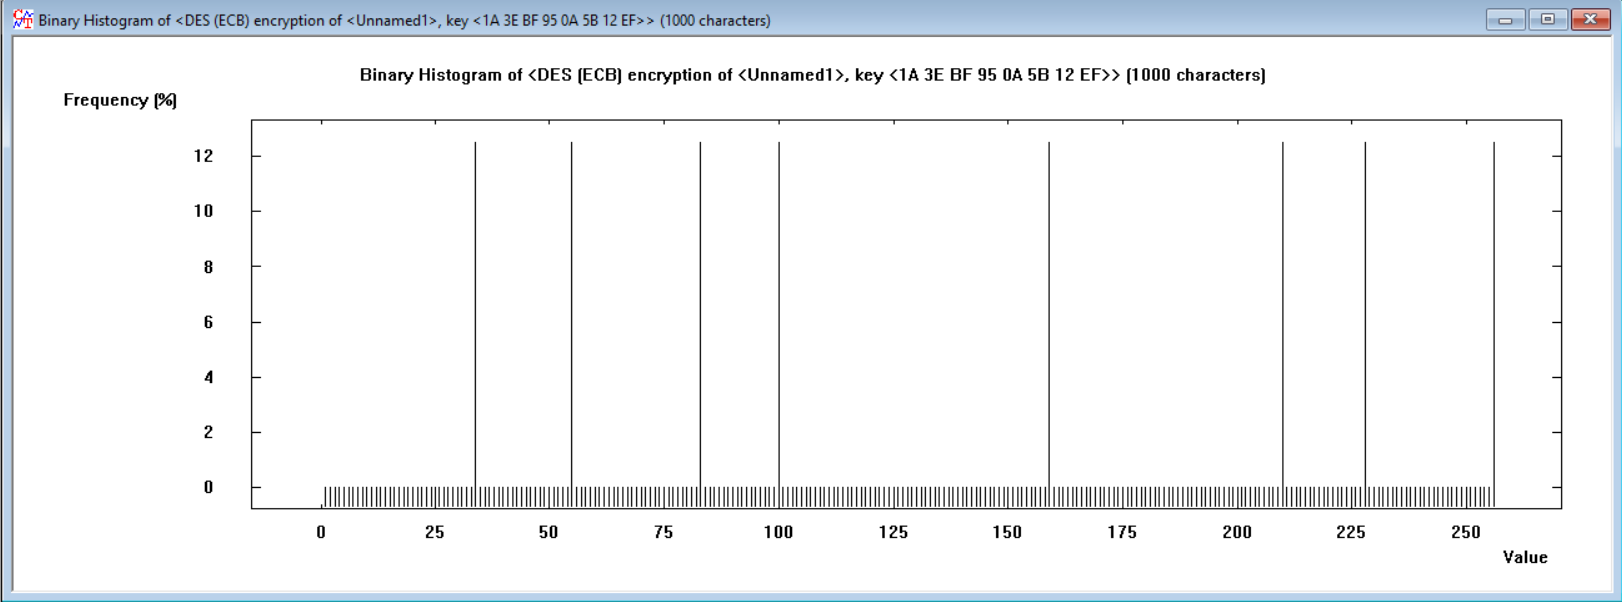
\includegraphics[width=0.8\textwidth]{cat_des_ecb_histogram.png}
    \caption{Histogram dla DES w trybie ECB}
\end{figure}

\begin{figure}[H]
    \centering
    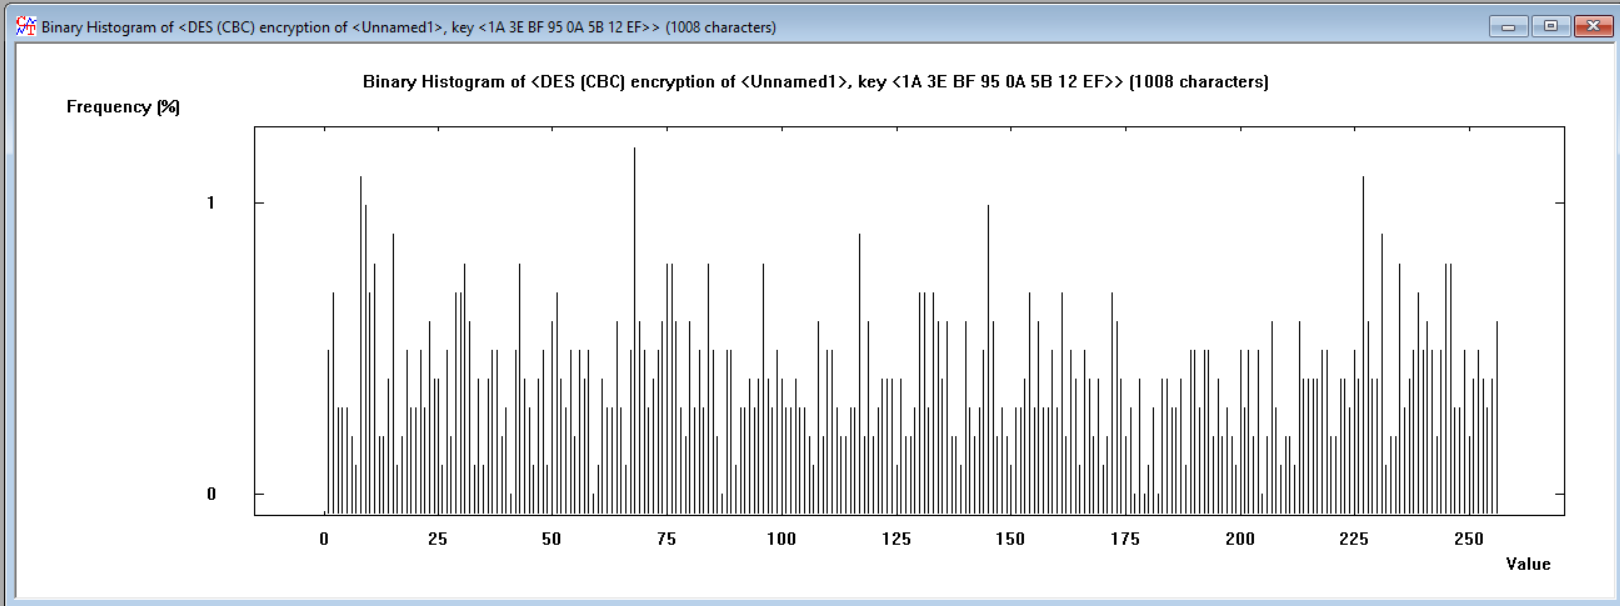
\includegraphics[width=0.8\textwidth]{cat_des_cbc_histogram.png}
    \caption{Histogram dla DES w trybie CBC}
\end{figure}

\begin{figure}[H]
    \centering
    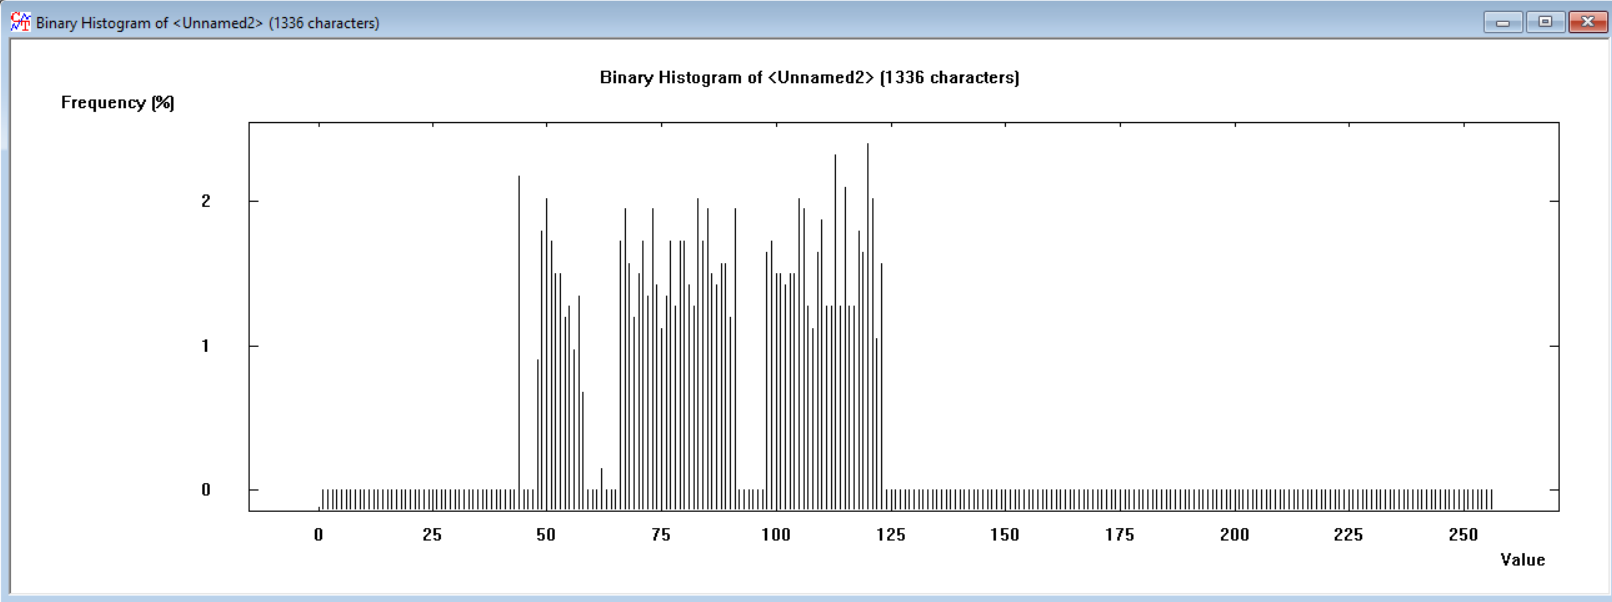
\includegraphics[width=0.8\textwidth]{cat_des_ofb_histogram.png}
    \caption{Histogram dla DES w trybie OFB}
\end{figure}


\begin{figure}[H]
    \centering
    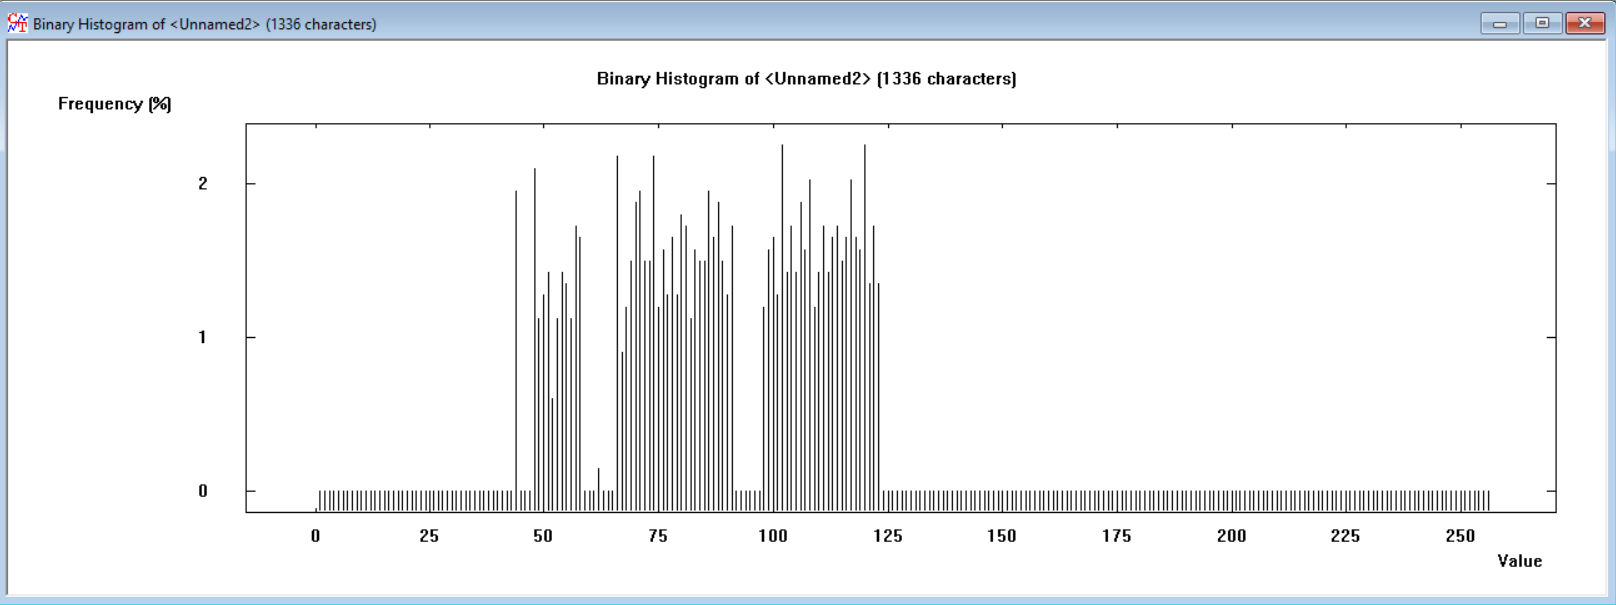
\includegraphics[width=0.8\textwidth]{cat_des_cbf_histogram.png}
    \caption{Histogram dla DES w trybie CFB}
\end{figure}

\begin{table}[H]
    \centering
    \caption{Entropia dla różnych trybów pracy DES}
    \begin{tabular}{|c|c|}
        \hline
        Tryb pracy & Entropia \\ \hline
        TJ & 2.00 (4.7) \\ \hline
        ECB & 3.00 (8.0) \\ \hline
        CBC & 7.76 (8.0)\\ \hline
        OFB & 5.97 (8.0) \\ \hline
        CFB & 4.68 (8.0) \\ \hline
    \end{tabular}
\end{table}
\subsection{Zadanie 2.4}

\begin{figure}[H]
    \centering
    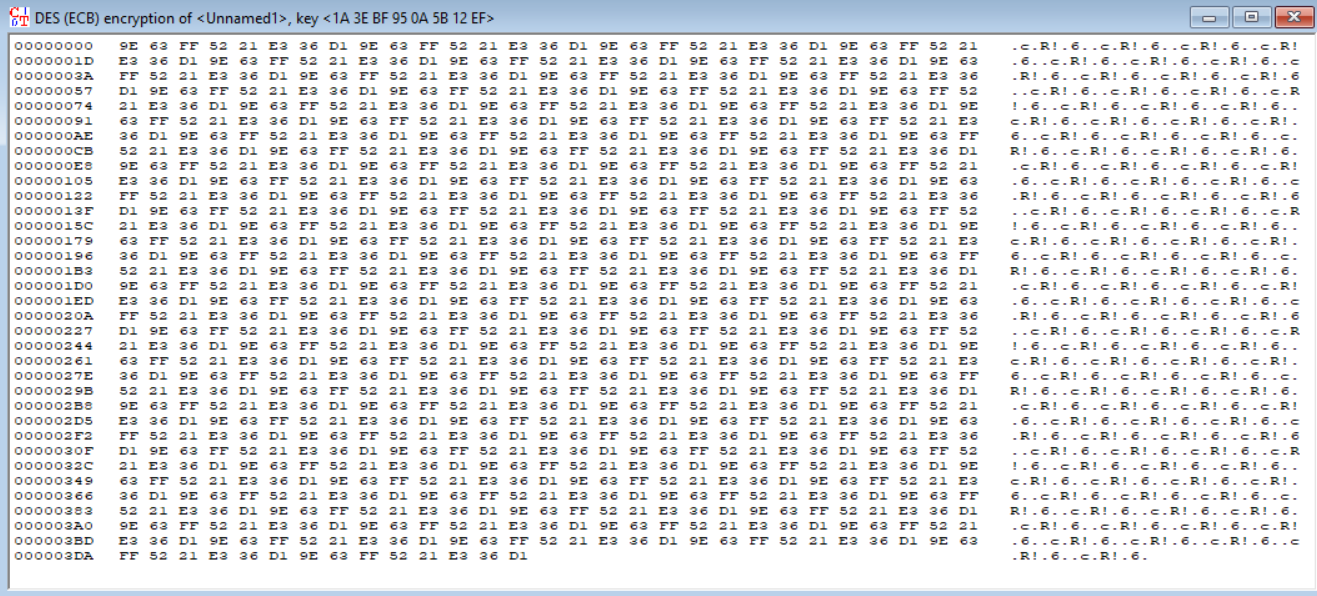
\includegraphics[width=0.8\textwidth]{cat_des_ecb.png}
    \caption{Kryptogram dla DES w trybie ECB}
\end{figure}

\begin{figure}[H]
    \centering
    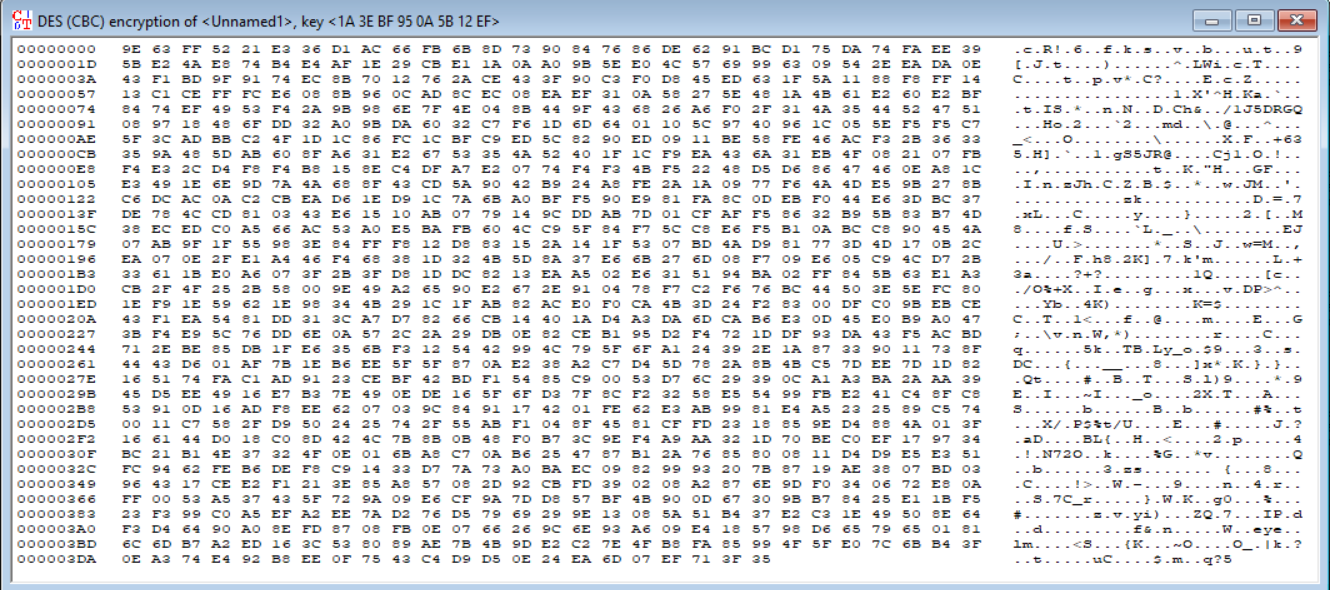
\includegraphics[width=0.8\textwidth]{car_des_cbc.png}
    \caption{Kryptogram dla DES w trybie CBC}
\end{figure}

\begin{figure}[H]
    \centering
    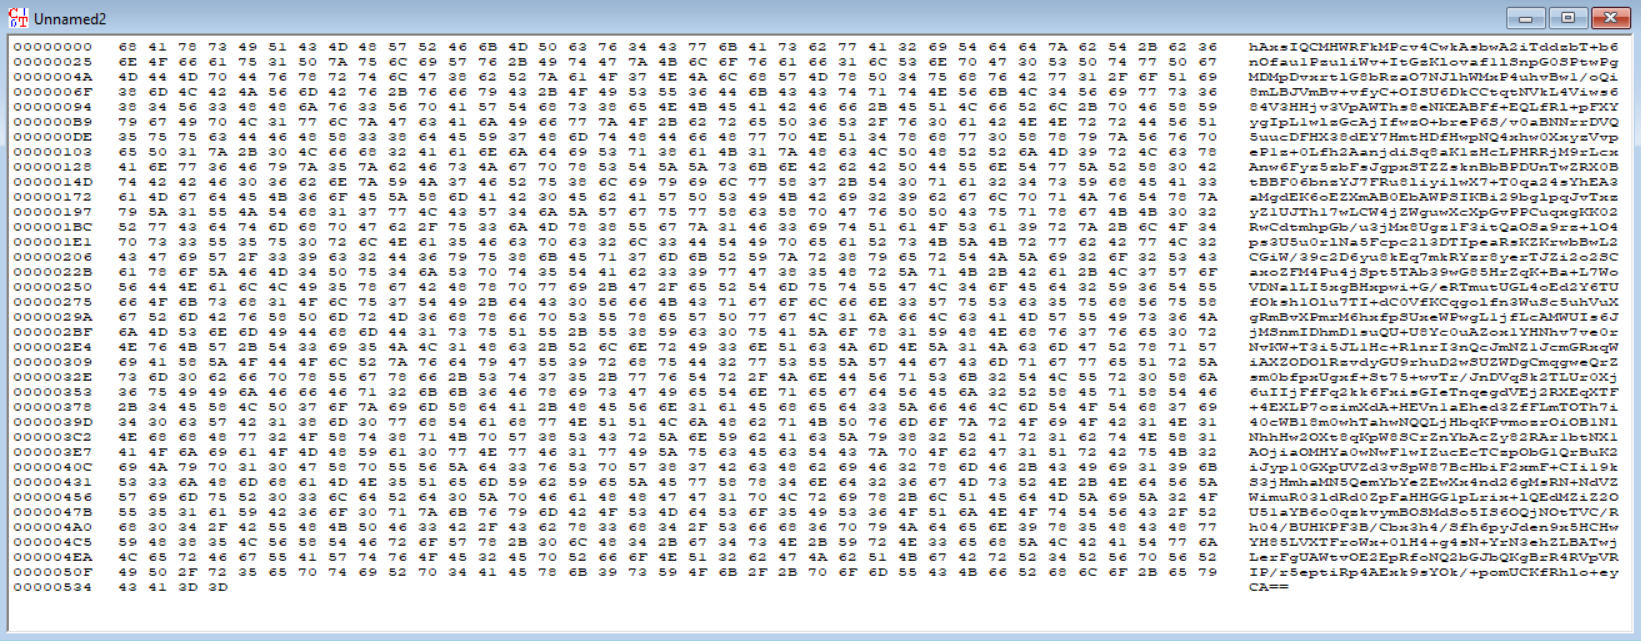
\includegraphics[width=0.8\textwidth]{cat_des_ofb.png}
    \caption{Kryptogram dla DES w trybie OFB}
\end{figure}


\begin{figure}[H]
    \centering
    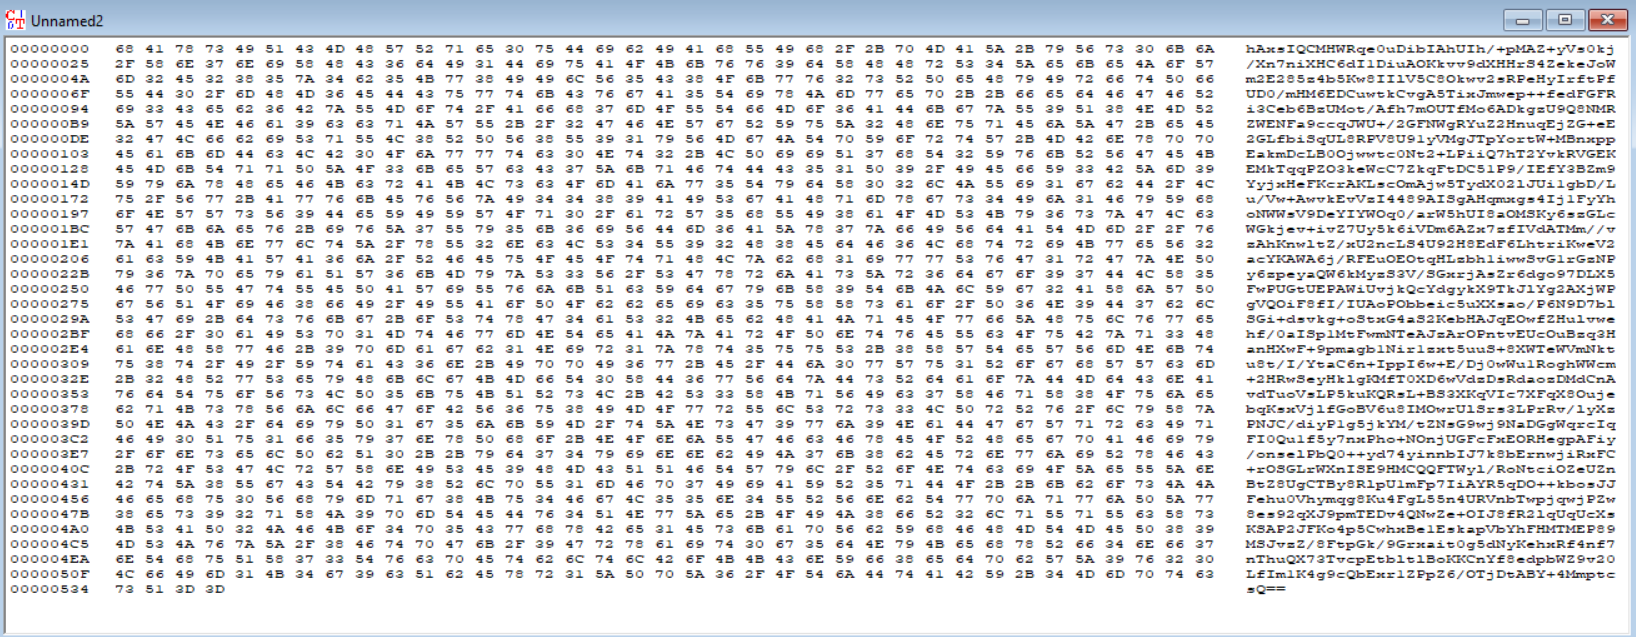
\includegraphics[width=0.8\textwidth]{cat_des_cbf.png}
    \caption{Kryptogram dla DES w trybie CBF}
\end{figure}




\textbf{Wnioski: } W przypadku algorytmu DES, tryb pracy ECB cechuje się powtarzalnością znaków kryptogramu, co można zauważyć gołym okiem jeśli tekst jawny nie był skomplikowany, oraz na histogramie widać wyraźe "górki" przy pewnych znakach.
Jeśli chodzi o tryb CBC, to kryptogram jest znacznie bardziej zróżnicowany, nie widać powtarzalności znaków, a entropia jest bardzo wysoka. Jeśli tekst jawny był do pewnego stopnia powtarzalny, skuteczniejszym i bezpieczniejszy trybem będzie
zdecydowanie tryb CBC, jeśli natomiast tekst był zróżnicowany, to tryb ECB również może być skuteczny, ale nie w takim stopniu jak CBC. Algorytmy OFB oraz CFB wydają się dawać podobne wyniki, w szczególności gdy przyjrzymy się na histogramy można zauważyć,
że w przypadku obu tych trybów dominują pewne 'grupy' znaków, podczas gdy pozostałe są kompletnie pomijane. Entropia dla tych trybów jest wyższa niż dla trybu ECB, lecz niższa niż dla CBC.

\subsection{Zadanie 2.5}
Do tego zadania został wykorzystany tekst zróżnicowany z pierwszj sekcji sprawozdania. Klucz wykorzystany do szyfrowania DES to \textbf{11 7C 39 27 1E 17 43 9E}, szyfrowanie AES za pomoca klucza \textbf{11 32 E1 3E 17 39 71 17 39 01 17 C3 92 71 E1 74}

\begin{itemize}
    \item Zmiana jednego bitu DES(ECB)
    \begin{figure}[H]
        \centering
        \label{fig:zmiana_jednego_bitu_ecb}
        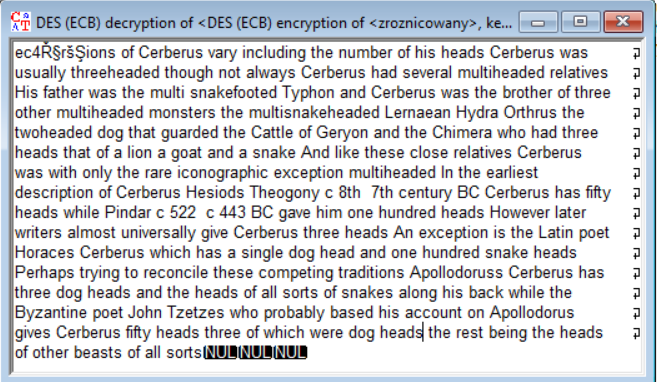
\includegraphics[width=0.8\textwidth]{zmiana_jednego_bitu.png}
    \end{figure}
    \item Zmiana jednego bitu DES(CBC)
    \begin{figure}[H]
        \centering
        \label{fig:zmiana_jednego_bitu_cbc}
        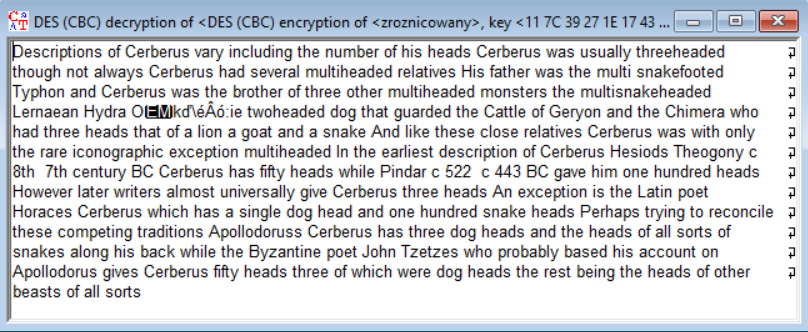
\includegraphics[width=0.8\textwidth]{zmiana_jednego_bitu_cbc.png}
    \end{figure}
    \item Zmiana kilku bitów DES(ECB)
    \begin{figure}[H]
        \centering
        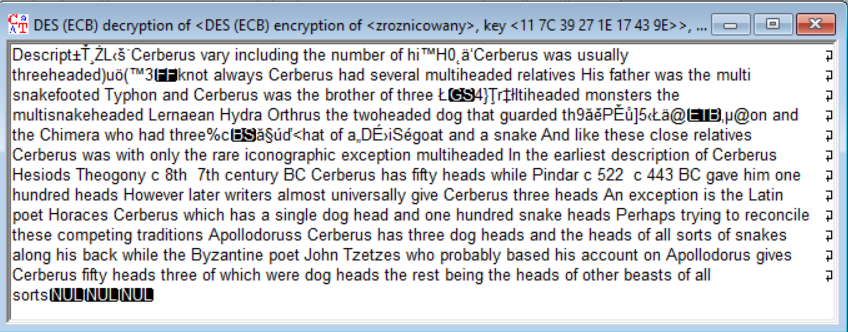
\includegraphics[width=0.8\textwidth]{zmiana_kilku_bitow.png}
    \end{figure}
    \item Zmiana kilku bitów DES(CBC)
    \begin{figure}[H]
        \centering
        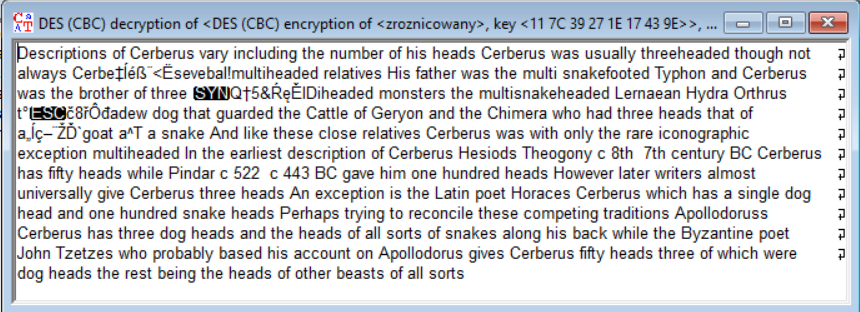
\includegraphics[width=0.8\textwidth]{zmiana_kilku_bitow_cbc.png}
    \end{figure}
    \item Usunięcie bajtu AES(ECB)
    \begin{figure}[H]
        \centering
        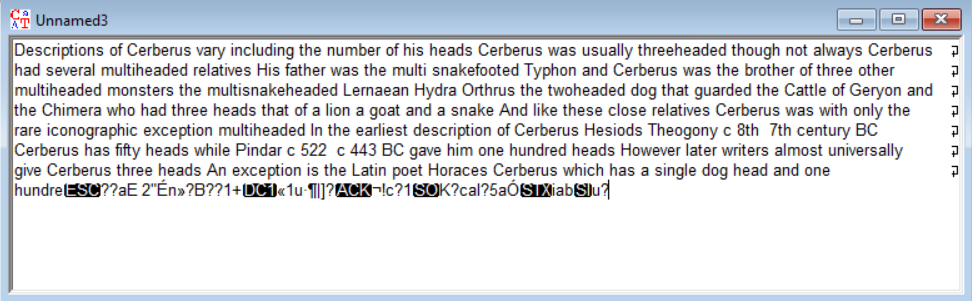
\includegraphics[width=0.8\textwidth]{usuniecie_ecb.png}
    \end{figure}
    \item Usunięcie bajtu AES(CBC)
    \begin{figure}[H]
        \centering
        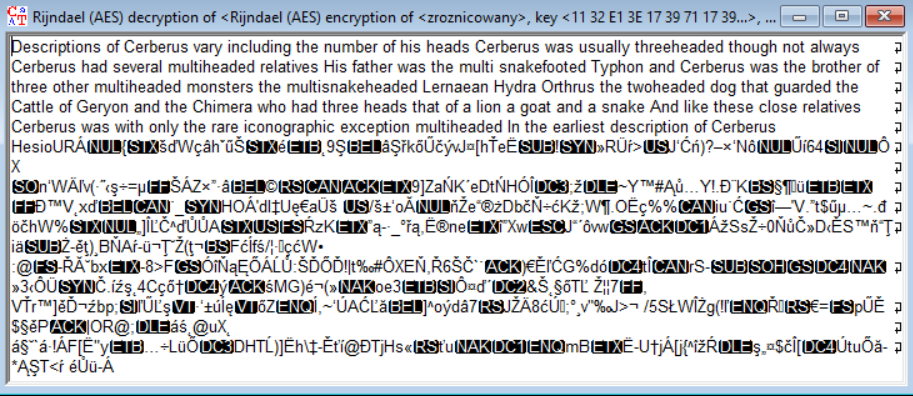
\includegraphics[width=0.8\textwidth]{usuniecie_cbc.png}
    \end{figure}
    \item Dodanie bajtu AES(ECB)
    \begin{figure}[H]
        \centering
        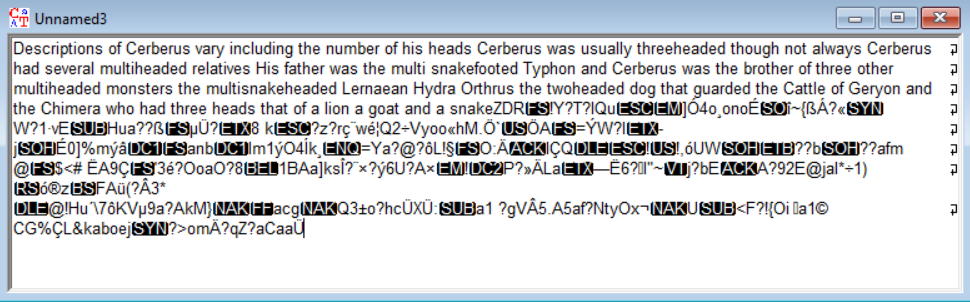
\includegraphics[width=0.8\textwidth]{dodanie_ecb.png}
    \end{figure}
    \item Dodanie bajtu AES(CBC)
    \begin{figure}[H]
        \centering
        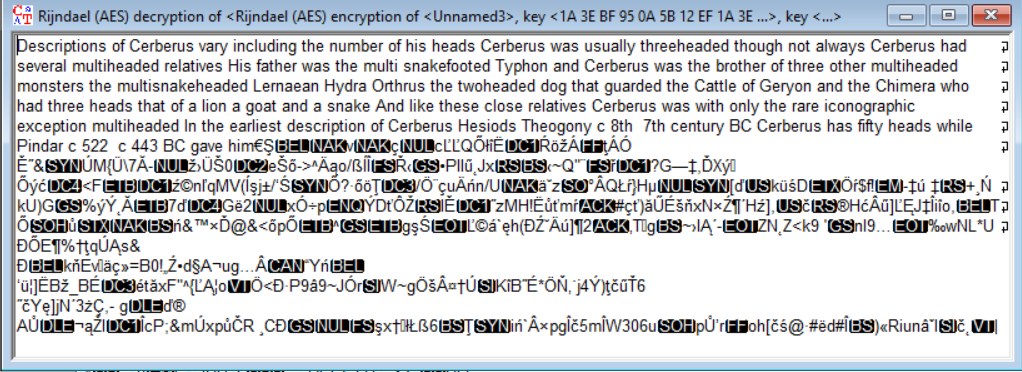
\includegraphics[width=0.8\textwidth]{dodanie_cbc.png}
    \end{figure}
\end{itemize}

\subsection{Pytanie 2.7}
    \textbf{Treść:} Jak wyglądają kryptogramy i ich entropie dla tekstu jawnego o jednorodnej strukturze
    w zależności od wybranego trybu szyfrowania? \\\\
    W zależności od wybranego trybu szyfrowania dostajemy kryptogram o różnym stopniu skomplikowania. W pzypadku użycia trybu ECB tekst tajny jest o wiele bardziej przewidywalny i cykliczny, zachowuje niską wartość entropii,
    a histogramy wyraźnie wskazują na dominację pewnych znaków nad innymi. Natomiast użycie trybu CBC sprawia że TT jest znacząco bardziej skomplikowany i losowy.
\subsection{Pytanie 2.8}
    \textbf{Treść:} Jak propagują się błędy z kryptogramu do tekstu jawnego przy deszyfracji TT z przekłamanym
    bitem/wieloma bitami (odpowiedź zilustruj odpowiednimi przykładami).\\\\
    W przypadku przekłamanego jednego bitu/ wielu biów w kryptogramie błąd propaguje się jedynie na jeden blok tekstu jawnego, w którym występuje przekłamany bit. Taka zmiana jest widoczna w przypadku trybu ECB jak i CBC co widać na
    rynukach w podpunkcie \ref{fig:zmiana_jednego_bitu_cbc}.
\subsection{Pytanie 2.9}
    \textbf{Treść:} Jak poszczególne tryby pracy algorytmów blokowych radzą sobie z utratą części wiadomości. Tzn.
    jaka jest możliwość odtworzenia TJ na podstawie TT z którego usunięto część zawartości (odpowiedź zilustruj odpowiednimi przykładami).\\\\
    W przypadku algorytmu AES pracującym w trybie ECB, usunięcie jednego bitu sprawiło, że cała wiadomość następująca po usuniętym bicie staje się niecztelna. 
    Dla trybu pracy CBC sytuacja jest analogiczna, lecz wiadomość staje się nieczytelna do momentu wystąpienia usuniętego bitu.
\subsection{Pytanie 2.10}
    \textbf{Treść:} Dla jakich zastosowań możemy wykorzystać tryby pracy: ECB, CBC?\\\\
    Tryb pracy CBC cechuje się większym skomplikowaniem niż ECB, lecz proces deszyfrowania trwa dłużej w związku z faktem, że
    tekst zaszyfrowany z użyciem CBC musi być szyfrowany w całości. ECB może być szyfrowany w częściach, co sprawia że jest wydajniejszy 'czasowo' i może być stosowany do 
    szyfrowania małej ilości danych. CBC jest za to bezpieczniejszy, lecz może wymagać więcej czasu w przypadku szyfrowania dużych plików ze względu na dodatkowe operacje.
\subsection{Pytanie 2.11}
    \textbf{Treść:} W przypadku których trybów proces szyfrowania/deszyfrowania można prowadzić równolegle?
    W przypadku którego trybu pracy można podzielić TT/TJ na kilka niezależnych części które będą deszyfrowane/szyfrowane
    równolegle na kilku komputerach, a następnie połączone dadzą ten sam rezultat co w przypadku realizowania całego procesu
    na jednym stanowisku.\\\\
    Tryb ECB umożliwa szyfrowanie oraz deszyfrowanie równolegle, ponieważ poszczególne bloki mogą być szyfrowane/deszyfrowane osobno, więc są od siebie niezależne.
    Natomiast tryb CBC sprawia, że cały tekst musi być poddany jednemu procesowi szyfrowania, ponieważ następne bloki tekstu są zależne od poprzednich. Natomiast proces deszyfrowania może zostać zrównoleglony.



\end{document}